\section{TEMPO}
\label{sec:method}

\subsection{Overall}
\label{sec:method:overview}
\begin{figure}[t]
    \centering
    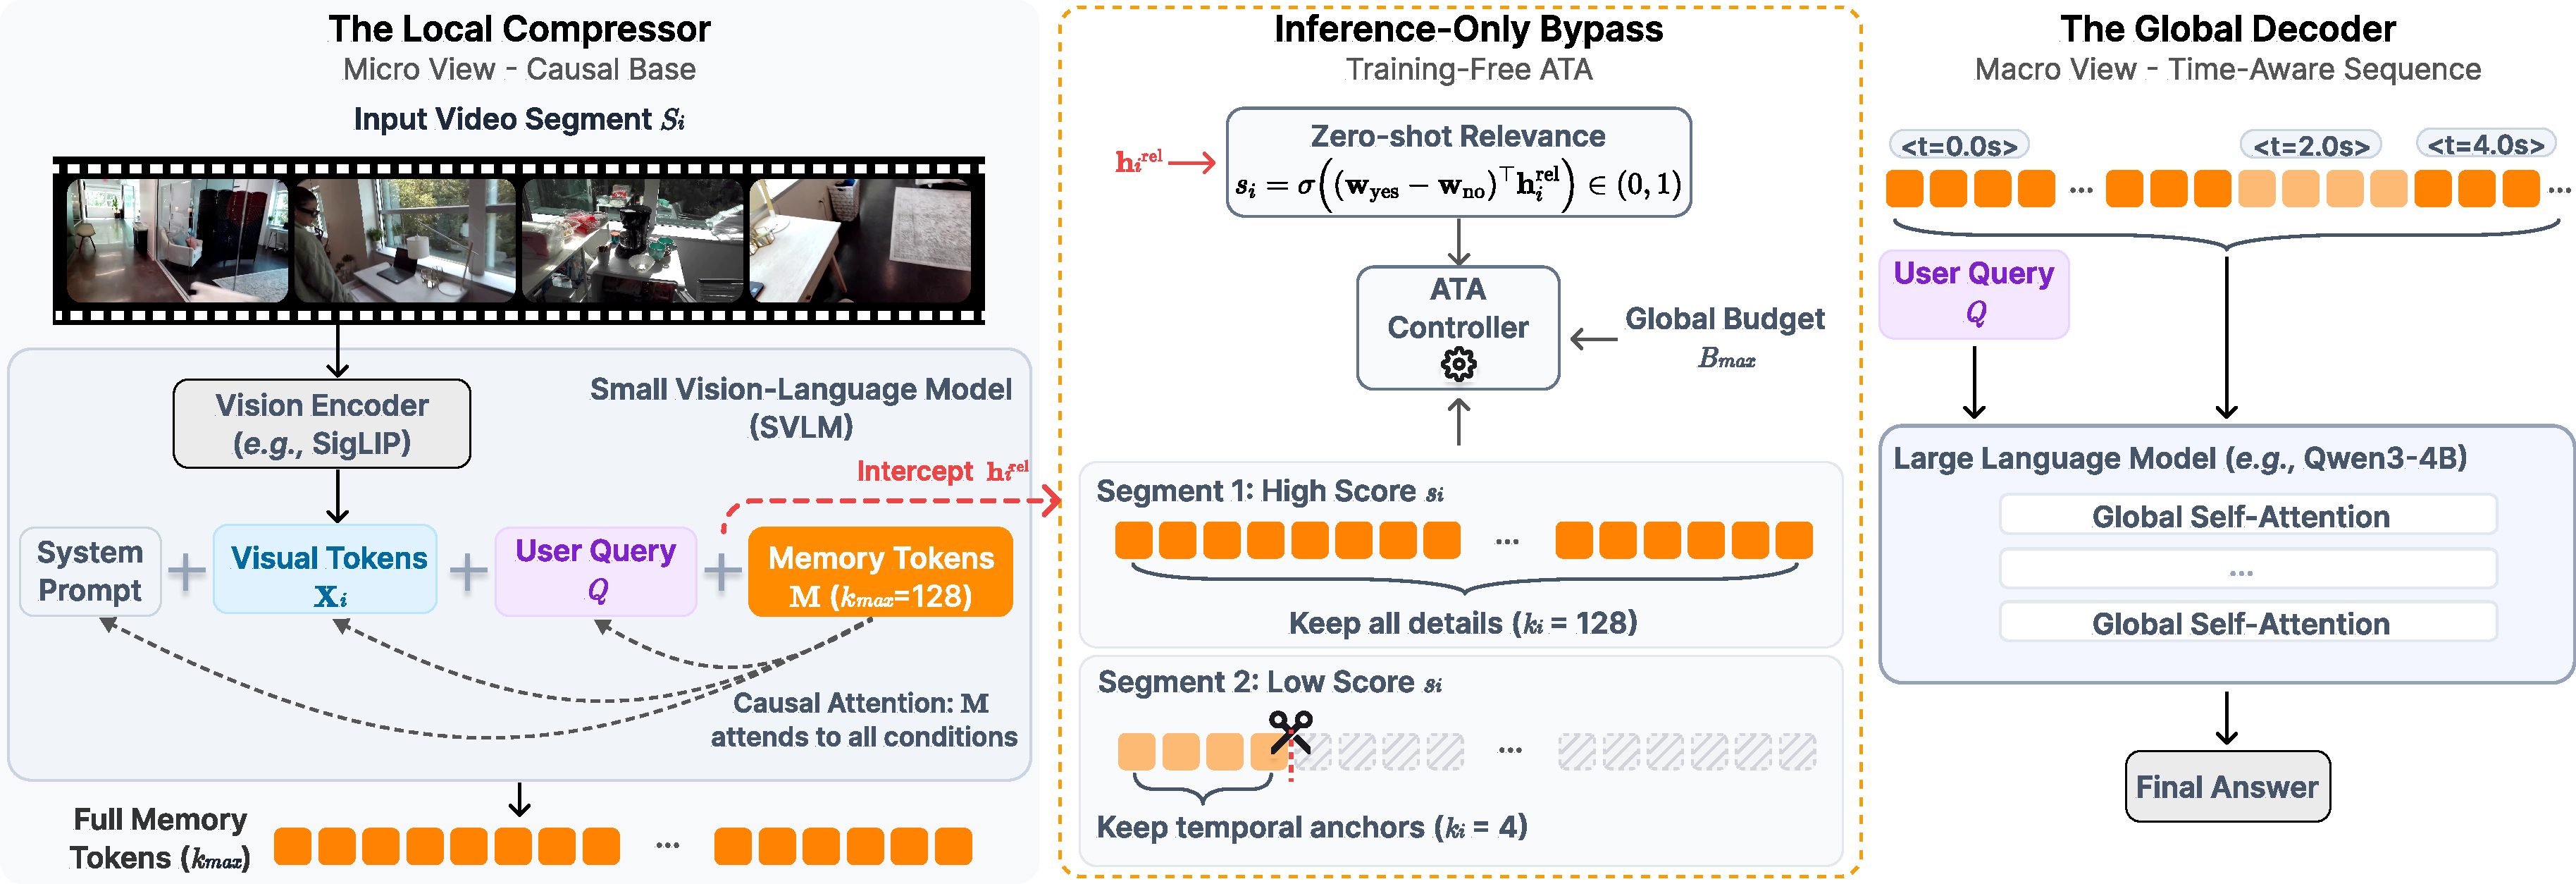
\includegraphics[width=\textwidth]{fig/tempo.pdf}
    \caption{
        \textbf{Overview of the Tempo framework.} 
        Our unified architecture casts long video understanding as an end-to-end, query-aware compression process. 
        \textbf{The Local Compressor (Left).} For each segment, a Small Vision-Language Model (SVLM) acts as a semantic temporal compressor. Under causal attention, learnable memory tokens $\mathbf{M}$ inherently distill the preceding visual tokens $\mathbf{X}_i$ and user query $Q$. 
        \textbf{Inference-Only Bypass (Middle).} During a single forward pass, an Adaptive Token Allocation (ATA) controller intercepts the hidden state $\mathbf{h}_i^{\mathrm{rel}}$ to compute a zero-shot relevance score $s_i$. This enables an $\mathcal{O}(1)$ dynamic head truncation, allocating dense bandwidth to query-critical segments while compressing redundancies into minimal temporal anchors to strictly satisfy a global budget $B_{\max}$. 
        \textbf{The Global Decoder (Right).} The compressed memory tokens are assembled into a highly sparse, time-aware sequence using explicit temporal tags (\eg, \texttt{<t=2.0s>}). A global LLM synthesizes this condensed multimodal context to generate the final response.
    }
    % \vspace{-0.8em}
    \label{fig:tempo}
\end{figure}


We target the fundamental bottleneck in long video MLLMs: the downstream LLM can only attend to a limited number of visual tokens, while hour-long videos produce a massive, continuous stream. Tempo resolves this mismatch by turning visual token reduction into an early cross-modal distillation problem.

\myparagraph{Problem Setup.}
Given a long video $\mathcal{V}$ and a user query $Q$, we uniformly partition $\mathcal{V}$ into $N$ temporal segments $\mathcal{S}=\{S_1,\dots,S_N\}$. Our goal is to convert each $S_i$ into a compact set of query-conditioned video memory tokens, with the total sequence bounded by a global inference budget~$B_{\max}$, enabling the downstream LLM to process the entire video and generate the final answer efficiently.

\myparagraph{Architecture.}
Tempo constitutes a two-level generative hierarchy (Fig.~\ref{fig:tempo}):
%
(1) an SVLM-based local compressor $\mathcal{C}_\phi$, and (2) an LLM-based global decoder $\mathcal{D}_\theta$.
%
Concretely, the SVLM's native vision encoder maps segment $S_i$ to dense visual tokens $\mathbf{X}_i$. Its causal attention then performs query-conditioned distillation, integrating $\mathbf{X}_i$ and query $Q$ into learnable memory tokens $\mathbf{M}$.
%
This yields a fixed-capacity representation $\mathbf{H}_i$ of exactly $k_{\max}$ tokens. A linear projector maps $\mathbf{H}_i$ into the LLM's embedding space as $\tilde{\mathbf{H}}_i$. Finally, the global LLM $\mathcal{D}_\theta$ consumes all memory tokens $\{\tilde{\mathbf{H}}_i\}_{i=1}^N$ alongside $Q$ to auto-regressively decode the answer.


\myparagraph{Two Phases: Training vs. Inference.}
Tempo is trained with a fixed per-segment capacity $k_{\max}$ to learn a strong query-aware local compressor $\mathcal{C}_\phi$. At inference, we additionally enforce a global budget $B_{\max}$. We therefore introduce ATA, a training-free strategy that uses a zero-shot relevance prior extracted from the same SVLM forward pass to allocate per-segment budgets $k_i \in [k_{\min}, k_{\max}]$, followed by a constant-time head truncation.

\subsection{Query-Aware Visual Compression}
\label{sec:method:compression}

We cast segment compression as a query-driven sequence-to-sequence transformation. An explicit information bottleneck forces the $\mathcal{C}_\phi$ to discard visual redundancies and distill semantic evidence relevant to user intent.

\myparagraph{SVLM Input Construction.}
For each segment $S_i$, the SVLM constructs a single causal sequence comprising: (i) a system prompt, (ii) visual tokens $\mathbf{X}_i$ (extracted via its native vision encoder), (iii) user query $Q$, and (iv) learnable memory tokens $\mathbf{M}$.
%
Placing $\mathbf{M}$ last is critical: under causal attention, each memory token inherently attends to all preceding visual and textual contexts. This conditions the SVLM to distill query-aligned evidence into $\mathbf{M}$. Extracting their final-layer hidden states yields the compressed representation $\mathbf{H}_i \in \mathbb{R}^{k_{\max}\times d_s}$.

\myparagraph{Sequence Assembly \& Temporal Grounding.}
To preserve temporal identity and causal order across the entire video, we prepend an explicit textual timestamp (\eg, \texttt{<t=2.0s>}) to each segment when assembling the global context. In practice, these temporal tags significantly stabilize long-range attribution (\emph{\ie, which evidence comes from where}) within the downstream global LLM.

\myparagraph{End-to-End Learning.}
Let the ground-truth answer be $A=\{a_t\}_{t=1}^{T}$. The global $\mathcal{D}_\theta$ receives all projected segment memories $\{\tilde{\mathbf{H}}_i\}_{i=1}^{N}$ in temporal order, optimized via standard auto-regressive next-token prediction:
%
\begin{equation}
    \mathcal{L}_{\mathrm{AR}}(\theta,\phi) = -\sum_{t=1}^{T}\log p_{\theta}\big(a_t \mid a_{<t}, Q, \{\tilde{\mathbf{H}}_i\}_{i=1}^{N}\big)
    \label{eq:loss}
\end{equation}
%
Crucially, we do not impose auxiliary compression losses, routing networks, or heuristic token-dropping regularizations during training. The fixed capacity of $k_{\max}$ memory tokens acts as a hard structural bottleneck. The gradients back-propagated from $\mathcal{L}_{\mathrm{AR}}$ naturally compel the compressor $\mathcal{C}_\phi$ to discard query-irrelevant backgrounds and pack the most predictive visual evidence into this bounded space.

\subsection{Zero-Shot Relevance Prior}
\label{sec:method:relevance}

A core insight driving Tempo is that modern multimodal foundation models (\eg, Qwen3-VL~\cite{bai2025qwen3}) inherently possess a robust zero-shot capability to evaluate semantic alignment between a visual sequence and a text query (Refer to Sec.~\ref{sec:exp:ablation} -- D). We harness this foundational prior to extract a highly accurate relevance signal without introducing or training any auxiliary routing modules.

\myparagraph{Logit-Based Relevance Score.}
To explicitly elicit this prior during inference, we slightly augment our training system prompt. Following the standard compression instruction, we append a strict binary directive: \emph{``Now, before compressing, answer exactly `Yes' or `No': is this segment relevant to the Query?''} Let $\mathbf{h}_i^{\mathrm{rel}} \in \mathbb{R}^{d_s}$ be the final hidden state immediately preceding the model's binary response. Using the SVLM's frozen language modeling head weights for the vocabulary tokens \texttt{Yes} ($\mathbf{w}_{\mathrm{yes}}$) and \texttt{No} ($\mathbf{w}_{\mathrm{no}}$), we compute a continuous relevance probability $s_i$ via logit difference~\cite{li2026qwen3}:
%
\begin{equation}
s_i = \sigma\Big( (\mathbf{w}_{\mathrm{yes}}-\mathbf{w}_{\mathrm{no}})^\top \mathbf{h}_i^{\mathrm{rel}} \Big) \in (0,1),
\label{eq:relevance}
\end{equation}
%
where $\sigma(\cdot)$ is the \texttt{Sigmoid} function. This $O(1)$ projection avoids auto-regressive decoding overhead while yielding a highly stable ranking signal.

\myparagraph{Single-Pass Design.}
The score $s_i$ and the compressed memory tokens $\mathbf{H}_i$ are extracted within a single forward pass of $\mathcal{C}_\phi$. As illustrated in the \emph{Inference-Only Bypass} (Fig.~\ref{fig:tempo}), we simply intercept the hidden state $\mathbf{h}_i^{\mathrm{rel}}$ to compute the zero-shot score, and then seamlessly continue the forward pass to extract $\mathbf{H}_i$. This architectural elegance guarantees that both the relevance routing signal and the compressed representations are rigorously conditioned on the exact same multimodal context, achieving adaptive evaluation with effectively zero latency.

\subsection{Adaptive Token Allocation (ATA)}
\label{sec:method:ata}

At inference, the total visual context provided to the global LLM must strictly satisfy a bounded capacity~$B_{\max}$. As illustrated in Fig.~\ref{fig:tempo}, the ATA controller translates the zero-shot scores $\{s_i\}$ into dynamic per-segment token budgets $k_i$, executing the physical compression via zero-overhead head truncation.

\myparagraph{Stage 1: Contrastive Linear Allocation.}
To guarantee causal continuity across the entire video sequence, we enforce a minimal temporal anchor for every segment, regardless of its relevance. We first normalize the raw scores via Min-Max scaling: $\hat{s}_i = (s_i-\min(\mathbf{s})) / (\max(\mathbf{s})-\min(\mathbf{s})+\epsilon)$. To maximize the contrast between query-critical events and irrelevant backgrounds, we linearly map these normalized scores to a target capacity:
%
\begin{equation}
k_i^{\mathrm{ideal}} = k_{\min} + \lfloor (k_{\max}-k_{\min}) \cdot \hat{s}_i \rfloor.
\label{eq:ideal_alloc}
\end{equation}

\myparagraph{Stage 2: Capacity-Aware Protection.}
Let $B_{\mathrm{base}}=N\cdot k_{\min}$ represent the foundational cost required to maintain the global temporal anchors. If the sum of ideal allocations satisfies the global limit ($\sum_i k_i^{\mathrm{ideal}} \le B_{\max}$), we directly adopt $\{k_i^{\mathrm{ideal}}\}$ to maximize sparsity. Otherwise, we distribute the residual budget $B_{\mathrm{res}}=B_{\max}-B_{\mathrm{base}}$ proportionally based on the normalized scores:
\begin{equation}
k_i = k_{\min} + \left\lfloor B_{\mathrm{res}} \cdot \frac{\hat{s}_i}{\sum_{j=1}^{N}\hat{s}_j+\epsilon} \right\rfloor.
\label{eq:soft_alloc}
\end{equation}
We then discretize $\{k_i\}$ and distribute any fractional remainders to strictly ensure $\sum_i k_i \le B_{\max}$ (Alg.~\ref{alg:ata}).

% \begin{algorithm}[t]
% \caption{Adaptive Token Allocation (ATA) at inference}
% \label{alg:ata}
% \KwIn{Segment memories $\{\mathbf{H}_i\}_{i=1}^N$, relevance scores $\{s_i\}_{i=1}^N$, budget $B_{\max}$, bounds $k_{\min},k_{\max}$}
% \KwOut{Budgeted memories $\{\mathbf{H}_i^{\mathrm{ATA}}\}_{i=1}^N$}
% Normalize $\{s_i\}\rightarrow\{\hat{s}_i\}$ by min-max scaling\;
% Compute $k_i^{\mathrm{ideal}}$ via Eq.~\eqref{eq:ideal_alloc}\;
% \eIf{$\sum_i k_i^{\mathrm{ideal}} \le B_{\max}$}{
% $k_i \leftarrow k_i^{\mathrm{ideal}}$\;
% }{
% $k_i \leftarrow$ Eq.~\eqref{eq:soft_alloc} with $B_{\mathrm{base}}=N k_{\min}$\;
% }
% Discretize $\{k_i\}$ to integers s.t.\ $\sum_i k_i \le B_{\max}$\;
% $\mathbf{H}_i^{\mathrm{ATA}} \leftarrow \mathbf{H}_i[1{:}k_i]$\;
% \Return{$\{\mathbf{H}_i^{\mathrm{ATA}}\}$}\;
% \end{algorithm}

\begin{algorithm}[t]
\caption{Adaptive Token Allocation (ATA) at inference}
\label{alg:ata}
\KwIn{Segment memories $\{\mathbf{H}_i\}_{i=1}^N$, relevance scores $\{s_i\}_{i=1}^N$, budget $B_{\max}$, bounds $k_{\min},k_{\max}$}
\KwOut{Budgeted memories $\{\mathbf{H}_i^{\mathrm{ATA}}\}_{i=1}^N$}
Normalize $\{s_i\}\rightarrow\{\hat{s}_i\}$ by min-max scaling\;
Compute $k_i^{\mathrm{ideal}}$ via Eq.~\eqref{eq:ideal_alloc}\;
\eIf{$\sum_i k_i^{\mathrm{ideal}} \le B_{\max}$}{
$k_i \leftarrow k_i^{\mathrm{ideal}}$\;
}{
$k_i \leftarrow$ Eq.~\eqref{eq:soft_alloc} with $B_{\mathrm{base}}=N k_{\min}$\;
}
Discretize $\{k_i\}$ to integers s.t.\ $\sum_i k_i \le B_{\max}$\;
$\mathbf{H}_i^{\mathrm{ATA}} \leftarrow \mathbf{H}_i[1{:}k_i], \quad \forall i \in \{1,\dots,N\}$\;
\Return{$\{\mathbf{H}_i^{\mathrm{ATA}}\}_{i=1}^N$}\;
\end{algorithm}

\myparagraph{Head Truncation: Zero-Overhead Token Selection.}
Once the dynamic budget $k_i$ is allocated, we compress the segment by simply slicing the memory sequence, \ie, $\mathbf{H}_i^{\mathrm{ATA}} = \mathbf{H}_i[1{:}k_i]$. Driven by the auto-regressive nature of the SVLM's causal attention, we empirically observe a semantic front-loading phenomenon: the local compressor packs the most salient global evidence into the earliest generated memory tokens (Refer to Sec.~\ref{sec:exp:ablation} -- C). Consequently, this $O(1)$ tensor slice naturally isolates high-value semantics without introducing lossy spatiotemporal pooling. The final global sequence $\{\tilde{\mathbf{H}}_i^{\mathrm{ATA}}\}_{i=1}^{N}$ strictly conforms to $B_{\max}$, rendering memory footprints entirely predictable even for hour-long reasoning. 